\chapter{Imunidade Inata e Inflamação}\label{ch:b3:innate-immunity}

Uma farpa sob a pele leva consigo dez mil bactérias que vão dobrar a
cada meia hora. Em minutos os vasos ao redor dilatam e vazam; em uma
hora os primeiros \omterm{def:b3:innate-immunity:innate}{neutrófilos} já se espremeram para fora do sangue e
rastejam rumo aos invasores ao longo de uma trilha química; em um dia o
local está vermelho, quente, inchado e dolorido --- os quatro sinais da
\omterm{def:b3:innate-immunity:inflammation}{inflamação} que Celso listou há dois mil anos --- e as bactérias estão
mortas, devoradas vivas por células que as reconheceram como estranhas
sem nunca as ter encontrado antes. Isto é a \omterm{def:b3:innate-immunity:innate}{imunidade inata}: a defesa
que todo animal tem, pronta antes da infecção, codificada no genoma em
vez de aprendida. Ela é rápida, é ela que mata a maioria dos invasores,
e é ela que avisa a imunidade aprendida, mais lenta, do próximo
capítulo de que há algo a aprender. Seus excessos --- o choque séptico,
a \omterm{def:b3:innate-immunity:inflammation}{inflamação} crônica, as febres das doenças autoinflamatórias --- são
tão instrutivos quanto seus êxitos.

\section{Camadas e células}

\begin{definition}[Imunidade inata]\label{def:b3:innate-immunity:innate}
\index{imunidade inata}\index{neutrófilo}\index{macrófago}\index{célula dendrítica}\index{célula natural killer}\index{barreira}
A \emph{imunidade inata} é o conjunto de defesas presentes antes de
qualquer exposição, codificadas por genes de linhagem germinativa que
não se rearranjam, que reconhecem características conservadas dos
micróbios em vez de indivíduos específicos, que agem em minutos a horas
e que (com ressalvas) não têm memória. Sua primeira camada são as
\emph{barreiras}: a queratina da pele, o muco e os \omterm{def:b3:cytoskeleton-motility:cilia}{cílios} das vias
aéreas, o ácido do estômago, o fluxo da urina e das lágrimas, a enzima
lisozima que corta o \omterm{def:b3:bacteriology:envelope}{peptidoglicano}, os \emph{peptídeos
antimicrobianos} (defensinas, catelicidinas) que perfuram as membranas
microbianas, e o \omterm{def:b3:microbiomes:symbiosis}{microbioma} comensal que ocupa os nichos
(\cref{ch:b3:microbiomes}). Suas células, todas da linhagem mieloide
exceto a última: os \emph{neutrófilos}, \qty{60}{\%} dos leucócitos do
sangue, $10^{11}$ produzidos por dia, vivendo um dia, os primeiros a
chegar e os principais matadores de bactérias; os \emph{macrófagos},
residentes longevos de todos os tecidos (células de Kupffer no fígado,
micróglia no cérebro, macrófagos alveolares no pulmão) que comem, fazem
a limpeza e dão o alarme; as \emph{células dendríticas}, que amostram os
tecidos e levam o que encontram aos linfonodos; os mastócitos, basófilos
e eosinófilos, armados contra parasitas e responsáveis pela alergia; e
as células \emph{natural killer} (NK), linfócitos que matam à primeira
vista células infectadas ou transformadas.
\end{definition}

\begin{proof}[Evidência]
Metchnikoff (1882), em Messina, enfiou um espinho de roseira numa larva
transparente de estrela-do-mar e viu, na manhã seguinte, células móveis
aglomeradas em volta dele; ele já tinha visto as mesmas células
englobarem partículas de alimento e grãos de corante, e propôs que
englobavam micróbios também --- os \emph{fagócitos}, agentes de uma
defesa do hospedeiro que ele passou a rastrear em todo animal que
conseguiu encontrar, da ameba ao homem. Dividiu o prêmio Nobel de 1908
com Ehrlich, cujos anticorpos representavam a visão oposta, humoral;
ambos tinham razão, e um século depois as duas metades da imunidade se
revelaram um só sistema, com a metade inata instruindo a adaptativa.
\end{proof}

\begin{omfigure}
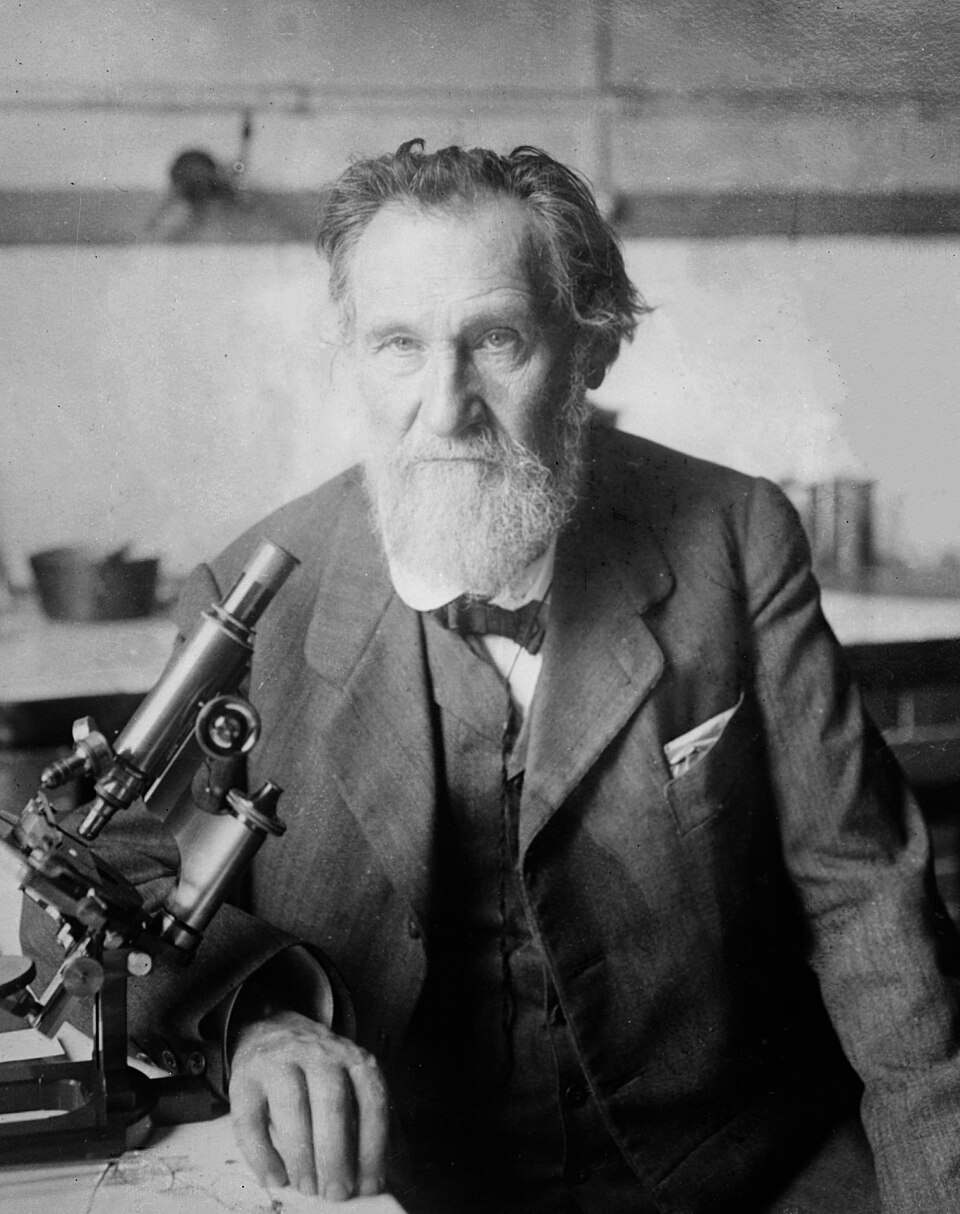
\includegraphics[width=0.30\linewidth]{images/book5/metchnikoff.jpg}\hspace{0.04\linewidth}
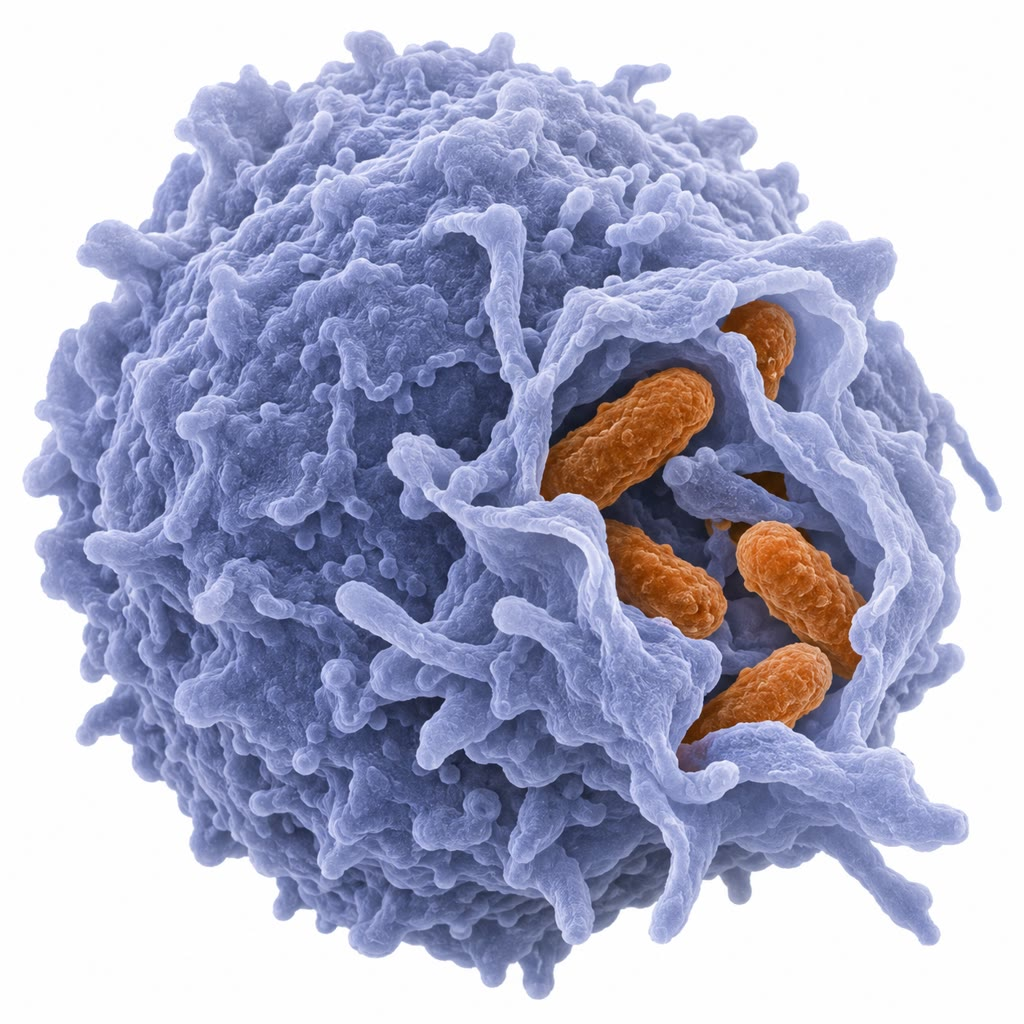
\includegraphics[width=0.30\linewidth]{images/book5/ai/b5-15-neutrophil-phagocytosis.jpg}\hspace{0.04\linewidth}
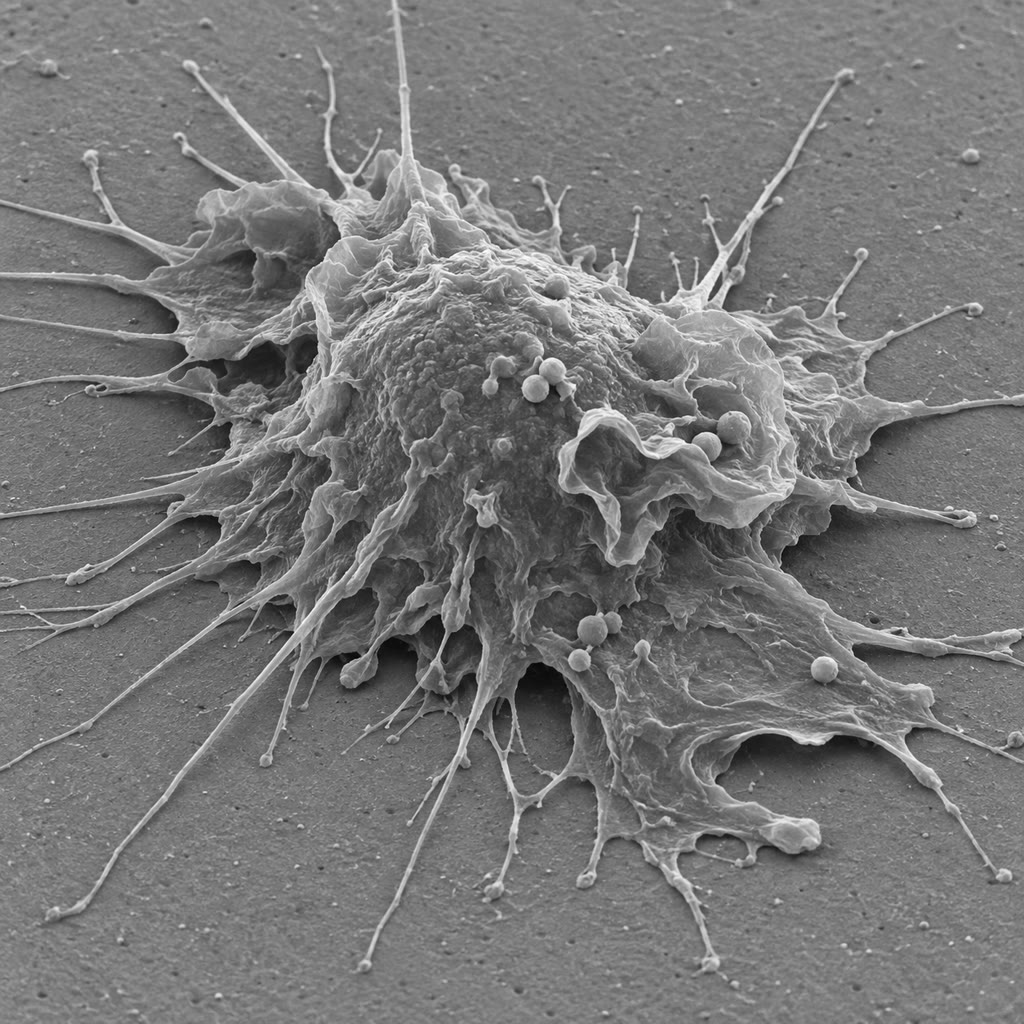
\includegraphics[width=0.30\linewidth]{images/book5/ai/b5-15-macrophage.jpg}

{\small Élie Metchnikoff, que observou fagócitos se juntarem em torno
de um espinho numa larva de estrela-do-mar e fundou a imunologia
celular (Library of Congress, domínio público). No centro: um
\omterm{def:b3:innate-immunity:innate}{neutrófilo} englobando bactérias. À direita: um \omterm{def:b3:innate-immunity:innate}{macrófago} espalhando
suas membranas ondulantes sobre uma superfície.}
\end{omfigure}

\section{Reconhecer o inimigo}

\begin{definition}[Reconhecimento de padrões]\label{def:b3:innate-immunity:prr}
\index{receptor de reconhecimento de padrões}\index{padrão molecular associado a patógenos}\index{receptor do tipo Toll}\index{padrão molecular associado a danos}\index{inflamassomo}
As células inatas reconhecem \emph{padrões moleculares associados a
patógenos} (PAMPs): moléculas comuns a classes inteiras de micróbios,
essenciais para eles e ausentes no hospedeiro --- o \omterm{def:b3:bacteriology:envelope}{lipopolissacarídeo}
das paredes \omterm{def:b3:bacteriology:envelope}{Gram-negativas}, o \omterm{def:b3:bacteriology:envelope}{peptidoglicano} e o ácido lipoteicoico das
\omterm{def:b3:bacteriology:envelope}{Gram-positivas}, a flagelina, os $\beta$-glicanos fúngicos, o RNA de
fita dupla, o RNA sem capuz 5$'$, o DNA com \omterm{def:b3:chromatin-epigenetics:methylation}{CpG} não metilado, o DNA no
citosol. Os receptores são os \emph{receptores de reconhecimento de
padrões} (PRRs), algumas dezenas ao todo, cada um codificado por um
gene: os \emph{receptores do tipo Toll} (TLRs) na superfície e nos
\omterm{def:b3:membrane-traffic:endocytosis}{endossomos} (TLR4 para o \omterm{def:b3:bacteriology:envelope}{lipopolissacarídeo}, TLR5 para a flagelina, TLR3
para o RNA de fita dupla, TLR9 para o DNA \omterm{def:b3:chromatin-epigenetics:methylation}{CpG}); as proteínas
citosólicas NOD para fragmentos de \omterm{def:b3:bacteriology:envelope}{peptidoglicano}, RIG-I para o RNA
viral, cGAS--STING para o DNA citosólico; as lectinas do tipo C para os
açúcares fúngicos. Os mesmos receptores, ou outros das mesmas famílias,
reconhecem \emph{padrões moleculares associados a danos} (DAMPs)
liberados por células lesadas --- ATP, ácido úrico, a proteína nuclear
HMGB1, DNA mitocondrial ---, de modo que uma lesão estéril também
inflama. A ligação ativa os fatores de transcrição NF-$\kappa$B e os
fatores reguladores de interferon, que ligam \omterm{def:b3:innate-immunity:inflammation}{citocinas}, \omterm{def:b3:innate-immunity:inflammation}{quimiocinas},
moléculas de adesão e genes antimicrobianos em menos de uma hora; um
subconjunto dos sensores citosólicos monta o \emph{inflamassomo}, uma
plataforma que ativa a caspase-1 para cortar a interleucina-1$\beta$ em
sua forma ativa e disparar a morte inflamatória chamada \omterm{def:b3:cell-cycle-apoptosis:other}{piroptose}
(\cref{ch:b3:cell-cycle-apoptosis}).
\end{definition}

\begin{proof}[Evidência]
Janeway propôs em 1989 que o sistema imune adaptativo não responde ao
antígeno sozinho, mas precisa de um sinal de receptores inatos que
tenham reconhecido padrões microbianos --- a explicação de por que as
vacinas precisam de adjuvantes, ``o segredinho sujo do imunologista''.
Hoffmann (1996) descobriu que \emph{Drosophila} sem o receptor Toll,
conhecido por seu papel no padrão embrionário, não conseguia montar uma
resposta antifúngica e morria coberta de mofo; Beutler (1998) mapeou a
resistência ao \omterm{def:b3:bacteriology:envelope}{lipopolissacarídeo} de uma linhagem de camundongos, que
sobrevivia a doses de endotoxina letais para as demais e não conseguia
eliminar infecções por \omterm{def:b3:bacteriology:envelope}{Gram-negativas}, até uma mutação no homólogo de
mamífero TLR4. O receptor da endotoxina, procurado por cinquenta anos,
era um Toll.
\end{proof}

\begin{omfigure}
\begin{tikzpicture}[every node/.style={font=\scriptsize}, >=stealth]
  % membrane
  \draw[very thick, omDef] (0,3.0) -- (11.5,3.0); \draw[very thick, omDef] (0,2.7) -- (11.5,2.7);
  \node[above] at (0.5,3.05) {fora}; \node[below] at (0.5,2.65) {citosol};
  % TLR4 with LPS
  \draw[thick, fill=omProp!35] (2.2,2.4) rectangle (2.6,3.9); \draw[thick, fill=omProp!35] (2.9,2.4) rectangle (3.3,3.9);
  \fill[omThm] (2.75,4.1) circle (0.14); \node[above] at (2.75,4.25) {LPS (um PAMP)};
  \node[right, align=left] at (3.4,3.5) {dímero de TLR4\\com MD2};
  % signalling
  \node[draw, thick, rounded corners, fill=omDef!20] (myd) at (2.75,1.7) {MyD88, quinases};
  \node[draw, thick, rounded corners, fill=omDef!20] (nfkb) at (2.75,0.6) {NF-$\kappa$B liberado};
  \node[draw, thick, rounded corners, fill=omMeth!25, align=center] (genes) at (2.75,-0.8) {TNF, IL-1$\beta$, IL-6, IL-8;\\moléculas de adesão; iNOS};
  \draw[->, thick] (2.75,2.4) -- (myd); \draw[->, thick] (myd) -- (nfkb); \draw[->, thick] (nfkb) -- (genes);
  \node[right, font=\tiny] at (3.3,1.2) {em menos de uma hora};
  % cytosolic sensors
  \node[draw, thick, rounded corners, fill=omProp!25, align=center] (rig) at (6.9,1.9) {RIG-I: RNA viral\\cGAS--STING: DNA citosólico};
  \node[draw, thick, rounded corners, fill=omMeth!25] (ifn) at (6.9,-0.2) {interferon do tipo I};
  \draw[->, thick] (rig) -- node[midway, right] {IRF3, IRF7} (ifn);
  \node[draw, thick, rounded corners, fill=omThm!20, align=center] (nlrp) at (10.9,1.9) {inflamassomo NLRP3:\\cristais, ATP, poros};
  \node[draw, thick, rounded corners, fill=omMeth!25, align=center] (il1) at (10.9,-0.8) {caspase-1: IL-1$\beta$\\liberada; piroptose};
  \draw[->, thick] (nlrp) -- (il1);
  \draw[->, thick, dashed] (genes.south) -- ++(0,-0.5) -| (il1.south) node[pos=0.25, below, font=\tiny] {pró-IL-1$\beta$ fornecida pela via do TLR};
\end{tikzpicture}

{\small Três braços do reconhecimento de padrões. Um \omterm{def:b3:innate-immunity:prr}{receptor do tipo
Toll} de superfície ligado ao \omterm{def:b3:bacteriology:envelope}{lipopolissacarídeo} sinaliza através do
NF-$\kappa$B até as \omterm{def:b3:innate-immunity:inflammation}{citocinas} inflamatórias; sensores citosólicos de
ácido nucleico viral induzem o interferon; o \omterm{def:b3:innate-immunity:prr}{inflamassomo} transforma o
precursor estocado da interleucina-1 na \omterm{def:b3:innate-immunity:inflammation}{citocina} ativa.}
\end{omfigure}

\begin{definition}[Complemento]\label{def:b3:innate-immunity:complement}
\index{complemento}\index{convertase de C3}\index{opsonização}\index{complexo de ataque à membrana}\index{anafilatoxina}
O \emph{complemento} é um sistema de cerca de trinta proteínas
plasmáticas, \qty{10}{\%} das globulinas do soro, que marca e destrói
micróbios por uma cascata de ativações proteolíticas. Três vias
convergem para a clivagem da proteína central C3: a via \emph{clássica},
iniciada pela C1q que se liga a anticorpos sobre uma superfície (ou à
\omterm{prop:b3:innate-immunity:systemic}{proteína C reativa}, ou a células apoptóticas); a via das
\emph{lectinas}, iniciada pela lectina ligante de manose que reconhece
açúcares microbianos; e a via \emph{alternativa}, em que a C3 se
hidrolisa espontaneamente a uma taxa baixa e a C3b resultante se prende
a qualquer superfície que encontre. Cada via constrói uma
\emph{convertase de C3}, uma enzima que cliva mais C3; a C3b que ela
deposita covalentemente sobre a superfície constrói, por sua vez, mais
convertase --- uma alça de amplificação ---, de modo que uma bactéria
fica revestida de milhões de C3b em minutos. A C3b é uma \emph{opsonina}:
os fagócitos têm receptores para ela e comem aquilo que ela reveste. Os
pequenos fragmentos C3a e C5a são \emph{anafilatoxinas} que dilatam
vasos, atraem \omterm{def:b3:innate-immunity:innate}{neutrófilos} e ativam mastócitos. E a C5b monta C6--C9 no
\emph{complexo de ataque à membrana}, um poro de \qty{10}{nm} que lisa
bactérias \omterm{def:b3:bacteriology:envelope}{Gram-negativas} e \omterm{def:b3:virology:virus}{vírus} envelopados. As células do hospedeiro
são poupadas porque carregam reguladores --- o fator H, o CD55, o CD59
--- que desmontam a convertase e bloqueiam o poro em suas próprias
superfícies; os micróbios, que não os têm, são consumidos pela alça.
\end{definition}

\begin{theorem}[A alça do complemento como discriminador cinético]\label{thm:b3:innate-immunity:complement}
\index{complemento!alça de amplificação}
Seja $B(t)$ o número de moléculas de C3b depositadas sobre uma
superfície. A C3b é depositada a uma pequena taxa constante $k_{0}$ pela
ativação espontânea da C3, e cada C3b depositada constrói convertase
que deposita mais, à taxa $a$ por C3b por segundo, enquanto os
reguladores (do hospedeiro) e o decaimento removem atividade de
convertase à taxa $d$ por C3b por segundo:
\[
\frac{\mathrm{d}B}{\mathrm{d}t} = k_{0} + (a - d)\,B .
\]
Sobre uma superfície em que $a > d$ --- um micróbio, sem reguladores
---, $B(t) = \bigl[k_{0}/(a-d)\bigr]\bigl(e^{(a-d)t} - 1\bigr)$ cresce
exponencialmente com constante de tempo $1/(a - d)$; sobre uma
superfície do hospedeiro, em que $d > a$, $B$ se aproxima do pequeno
valor estacionário $k_{0}/(d - a)$. As mesmas moléculas, nas mesmas
concentrações, depositam um milhão de C3b sobre uma bactéria em poucos
minutos e algumas dezenas sobre a célula ao lado dela: a distinção
entre o próprio e o não próprio não é feita pelo reconhecimento, mas
pelo sinal de $a - d$.
\end{theorem}
\begin{proof}
A equação é linear com coeficientes constantes. Para $a \ne d$ o ponto
fixo é $B^{*} = -k_{0}/(a-d)$; escrevendo $B = B^{*} + u$,
$\mathrm{d}u/\mathrm{d}t = (a-d)u$, de modo que $u = u_{0}e^{(a-d)t}$ e,
com $B(0) = 0$, $B(t) = \bigl[k_{0}/(a-d)\bigr](e^{(a-d)t} - 1)$. Para
$a > d$ isso cresce sem limite (até acabar a C3 ou a superfície); para
$a < d$ a exponencial decai e $B \to k_{0}/(d-a) > 0$. Com $k_{0} = 1$
por segundo e $a - d = \qty{0.1}{s^{-1}}$ numa bactéria, $B(\qty{2}{min})
= 10(e^{12} - 1) \approx 1.6\times 10^{6}$; com $d - a =
\qty{0.1}{s^{-1}}$ numa célula do hospedeiro, $B^{*} = 10$.
\end{proof}

\begin{omfigure}
\begin{tikzpicture}
\begin{axis}[
  width=0.66\linewidth, height=5.6cm,
  axis x line=bottom, axis y line=left,
  xmin=0, xmax=150, ymin=1, ymax=1e7, ymode=log,
  xlabel={segundos}, ylabel={C3b depositada},
  xlabel style={font=\small, at={(axis description cs:0.5,-0.12)}, anchor=north}, ylabel style={font=\small},
  tick label style={font=\small}, xtick={0,30,60,90,120,150},
  clip=false,
]
\addplot[very thick, omThm, domain=1:150, samples=80] {10*(exp(0.1*x)-1)};
\addplot[very thick, omDef, domain=1:150, samples=80] {10*(1-exp(-0.1*x))};
\node[font=\scriptsize, omThm, anchor=east] at (axis cs:100,2e5) {micróbio: $a > d$, exponencial};
\node[font=\scriptsize, omDef, anchor=south west] at (axis cs:60,14) {célula do hospedeiro: $d > a$, satura em $k_{0}/(d-a)$};
\end{axis}
\end{tikzpicture}

{\small A alça do \omterm{def:b3:innate-immunity:complement}{complemento} sobre duas superfícies, com $k_{0} = 1$
por segundo e $|a - d| = \qty{0.1}{s^{-1}}$: sobre um micróbio sem
reguladores a C3b cresce exponencialmente e chega a um milhão em dois
minutos; sobre uma célula do hospedeiro, com reguladores, estabiliza em
dez.}
\end{omfigure}

\begin{omfigure}
\begin{tikzpicture}[every node/.style={font=\scriptsize}, >=stealth]
  \node[draw, thick, rounded corners, fill=omDef!20, align=center] (cl) at (-4.2,3.0) {clássica:\\C1q sobre anticorpo\\ou proteína C reativa};
  \node[draw, thick, rounded corners, fill=omDef!20, align=center] (le) at (0,3.0) {das lectinas:\\lectina ligante de manose\\sobre açúcares microbianos};
  \node[draw, thick, rounded corners, fill=omDef!20, align=center] (al) at (4.2,3.0) {alternativa:\\ativação espontânea da C3,\\C3b em qualquer superfície};
  \node[draw, thick, rounded corners, fill=omProp!35, minimum width=3cm] (conv) at (0,1.2) {convertase de C3};
  \node[draw, thick, rounded corners, fill=omThm!25, align=center] (c3b) at (0,-0.4) {C3 $\to$ C3b (na superfície) $+$ C3a};
  \draw[->, thick] (cl) -- (conv); \draw[->, thick] (le) -- (conv); \draw[->, thick] (al) -- (conv);
  \draw[->, thick] (conv) -- (c3b);
  \draw[->, very thick, omThm] (c3b.east) .. controls (3.2,-0.4) and (3.2,1.2) .. (conv.east) node[pos=0.5, right, align=left] {alça de amplificação:\\a C3b constrói mais convertase};
  \node[draw, thick, rounded corners, fill=omMeth!25, align=center] (ops) at (-4.4,-2.2) {opsonização:\\os fagócitos comem\\o que a C3b reveste};
  \node[draw, thick, rounded corners, fill=omMeth!25, align=center] (ana) at (0,-2.2) {C3a, C5a:\\vasos dilatam, neutrófilos\\e mastócitos recrutados};
  \node[draw, thick, rounded corners, fill=omMeth!25, align=center] (mac) at (4.4,-2.2) {C5b--C9:\\complexo de ataque\\à membrana, lise};
  \draw[->, thick] (c3b) -- (ops); \draw[->, thick] (c3b) -- (ana); \draw[->, thick] (c3b) -- (mac);
  \node[draw, thick, rounded corners, fill=gray!15, align=center] (reg) at (-4.4,1.2) {reguladores do hospedeiro:\\fator H, CD55, CD59};
  \draw[-|, thick, gray!60!black] (reg) -- (conv);
\end{tikzpicture}

{\small O \omterm{def:b3:innate-immunity:complement}{complemento}. Três rotas constroem uma \omterm{def:b3:innate-immunity:complement}{convertase de C3}; a C3b
que ela deposita constrói mais (a alça do teorema), e a C3b depositada
opsoniza, os fragmentos inflamam e o complexo terminal lisa. As células
do hospedeiro carregam reguladores que cortam a alça (e, com o CD59,
bloqueiam o poro) em suas próprias membranas.}
\end{omfigure}

\section{Inflamação}

\begin{definition}[Inflamação aguda]\label{def:b3:innate-immunity:inflammation}
\index{inflamação}\index{citocina}\index{quimiocina}\index{extravasamento}\index{selectina}\index{integrina}
A \emph{inflamação} é a resposta de um tecido vascularizado à lesão ou à
infecção, orquestrada pelas \emph{citocinas} --- as pequenas proteínas
de sinalização das células imunes, aqui sobretudo o TNF, a
interleucina-1 e a interleucina-6 dos \omterm{def:b3:innate-immunity:innate}{macrófagos} ativados --- e pelas
\emph{quimiocinas}, as citocinas que dirigem a migração. Suas etapas
explicam os sinais de Celso. A histamina dos mastócitos, o óxido
nítrico e as prostaglandinas dilatam as arteríolas: \emph{rubor} e
\emph{calor}. O endotélio das vênulas se contrai e deixa vazar plasma,
cujas proteínas --- \omterm{def:b3:innate-immunity:complement}{complemento}, anticorpos, fatores de coagulação ---
inundam o tecido: \emph{tumor}. A bradicinina e a prostaglandina
E$_{2}$ sensibilizam as terminações nervosas: \emph{dor}. E os
leucócitos chegam por \emph{extravasamento}: o TNF e a interleucina-1
fazem o endotélio expor \emph{selectinas}, nas quais os \omterm{def:b3:innate-immunity:innate}{neutrófilos} que
passam se prendem e rolam; as quimiocinas (interleucina-8) na
superfície endotelial ativam as \emph{integrinas} dos \omterm{def:b3:innate-immunity:innate}{neutrófilos}, que
se ligam firmemente às moléculas de adesão endoteliais e param a
célula; e o \omterm{def:b3:innate-immunity:innate}{neutrófilo} se espreme entre as células endoteliais e segue
o gradiente de quimiocina até o tecido --- toda a sequência em poucos
minutos, a até um milhão de células por hora num local infectado.
\end{definition}

\begin{omfigure}
\begin{tikzpicture}[every node/.style={font=\scriptsize}, >=stealth]
  % vessel wall
  \fill[omThm!10] (0,0) rectangle (12,2.3); \node[left, omThm!70!black, anchor=north east] at (12,2.25) {sangue, fluindo $\rightarrow$};
  \foreach \x in {0,1.5,3,4.5,6,7.5,9,10.5} \draw[thick, fill=omDef!30] (\x,-0.05) rectangle (\x+1.45,0.35);
  \node[right] at (0.1,-0.35) {endotélio};
  \fill[omMeth!8] (0,-1.7) rectangle (12,-0.45); \node[right, omMeth!60!black] at (0.1,-1.55) {tecido};
  % bacteria and chemokine gradient
  \foreach \p in {(10.6,-1.1),(11.0,-0.9),(11.3,-1.2)} \fill[omProp] \p ellipse (0.14 and 0.07);
  \node[below, omProp] at (11.0,-1.35) {bactérias};
  \node[below, font=\tiny] at (8.0,-0.5) {gradiente de quimiocina $\rightarrow$};
  % neutrophils in sequence
  \draw[thick, fill=white] (1.2,1.1) circle (0.3); \node[above] at (1.2,1.45) {1. fluindo};
  \draw[thick, fill=white] (3.4,0.68) circle (0.3); \node[above] at (3.4,1.05) {2. rolando nas selectinas};
  \draw[omThm, thick] (3.1,0.45) -- (3.05,0.35); \draw[omThm, thick] (3.4,0.38) -- (3.4,0.35); \draw[omThm, thick] (3.7,0.45) -- (3.75,0.35);
  \draw[thick, fill=white] (6.0,0.62) ellipse (0.38 and 0.26); \node[above, align=center] at (6.0,0.95) {3. adesão firme\\(integrinas)};
  \draw[thick, fill=white] (8.25,0.18) ellipse (0.2 and 0.42); \node[above, align=center] at (8.4,0.95) {4. espremendo-se\\entre as células};
  \draw[thick, fill=white] (9.6,-1.0) circle (0.3); \node[left] at (9.25,-1.0) {5. rastejando até o local};
  \draw[->, thick, gray] (1.5,1.05) -- (3.0,0.8); \draw[->, thick, gray] (3.7,0.68) -- (5.6,0.62); \draw[->, thick, gray] (6.4,0.5) -- (8.0,0.4); \draw[->, thick, gray] (8.3,-0.3) -- (9.3,-0.8);
  % TNF label
  \node[below, align=center, font=\tiny] at (4.0,-1.75) {o TNF e a IL-1 dos macrófagos teciduais fazem o endotélio expor\\as selectinas e moléculas de adesão que prendem os neutrófilos};
\end{tikzpicture}

{\small O \omterm{def:b3:innate-immunity:inflammation}{extravasamento}. As \omterm{def:b3:innate-immunity:inflammation}{citocinas} dos \omterm{def:b3:innate-immunity:innate}{macrófagos} teciduais tornam
pegajosa a parede da vênula; um \omterm{def:b3:innate-immunity:innate}{neutrófilo} que passa se prende às
\omterm{def:b3:innate-immunity:inflammation}{selectinas} e rola, é parado por suas \omterm{def:b3:innate-immunity:inflammation}{integrinas}, espreme-se entre as
células endoteliais e segue o gradiente de \omterm{def:b3:innate-immunity:inflammation}{quimiocina} até as bactérias.}
\end{omfigure}

\begin{proposition}[A febre, a fase aguda e a resolução]\label{prop:b3:innate-immunity:systemic}
\index{febre}\index{resposta de fase aguda}\index{proteína C reativa}\index{resolução da inflamação}
A interleucina-1, o TNF e a interleucina-6 também agem à distância. No
hipotálamo induzem a prostaglandina E$_{2}$, que eleva o ponto de
ajuste da temperatura corporal: a \emph{febre}, que retarda muitas
bactérias, acelera as próprias reações das células imunes e custa cerca
de \qty{12}{\%} a mais de metabolismo por grau. No fígado induzem as
\emph{proteínas de fase aguda} --- a \omterm{prop:b3:innate-immunity:systemic}{proteína C reativa}, que se liga à
fosfocolina bacteriana, ativa o \omterm{def:b3:innate-immunity:complement}{complemento} e sobe mil vezes em dois
dias, a medida de \omterm{def:b3:innate-immunity:inflammation}{inflamação} do clínico; o fibrinogênio; a lectina
ligante de manose; e a hepcidina, que tranca o ferro longe dos
micróbios que dele precisam. Na medula liberam \omterm{def:b3:innate-immunity:innate}{neutrófilos} e aceleram
sua produção. A \omterm{def:b3:innate-immunity:inflammation}{inflamação} existe para acabar: à medida que o estímulo
é eliminado, os mediadores lipídicos passam das prostaglandinas às
lipoxinas e resolvinas, os \omterm{def:b3:innate-immunity:innate}{neutrófilos} morrem por \omterm{def:b3:cell-cycle-apoptosis:apoptosis}{apoptose} e são comidos
pelos \omterm{def:b3:innate-immunity:innate}{macrófagos}, que então passam a um programa de reparo, secretando
fatores de crescimento e interleucina-10 --- a \emph{resolução}. Quando
o estímulo persiste (um bacilo da tuberculose que não pode ser morto,
um cristal, um autoantígeno), a resposta se torna crônica: os \omterm{def:b3:innate-immunity:innate}{macrófagos}
muram o local num granuloma, os fibroblastos depositam cicatriz e o
tecido é destruído por sua própria defesa.
\end{proposition}

\begin{example}[Sepse]\label{ex:b3:innate-immunity:sepsis}
A \omterm{def:b3:innate-immunity:inflammation}{inflamação} confinada a uma farpa é uma cura; as mesmas reações por
todo o corpo são uma catástrofe. Quando bactérias ou seu
\omterm{def:b3:bacteriology:envelope}{lipopolissacarídeo} chegam ao sangue em quantidade, os \omterm{def:b3:innate-immunity:innate}{macrófagos} de
toda parte liberam TNF e interleucina-1 ao mesmo tempo: todos os vasos
dilatam e vazam, a pressão arterial despenca, a coagulação é ativada em
dez mil capilares e consome os fatores de coagulação, e os órgãos, sem
perfusão, falham --- o \emph{choque séptico}, que mata de um quarto a
metade daqueles a quem acomete, uns onze milhões de pessoas por ano.
Alguns microgramas de \omterm{def:b3:bacteriology:envelope}{lipopolissacarídeo} injetados num voluntário
produzem febre, calafrios e queda da pressão arterial em duas horas; um
camundongo sem TLR4 ignora uma dose cem vezes letal. A doença é a
resposta do hospedeiro, e os \omterm{def:b3:bacteriology:antibiotics}{antibióticos} que matam as bactérias podem
piorá-la por algumas horas, ao liberar mais endotoxina.
\end{example}

\begin{omfigure}
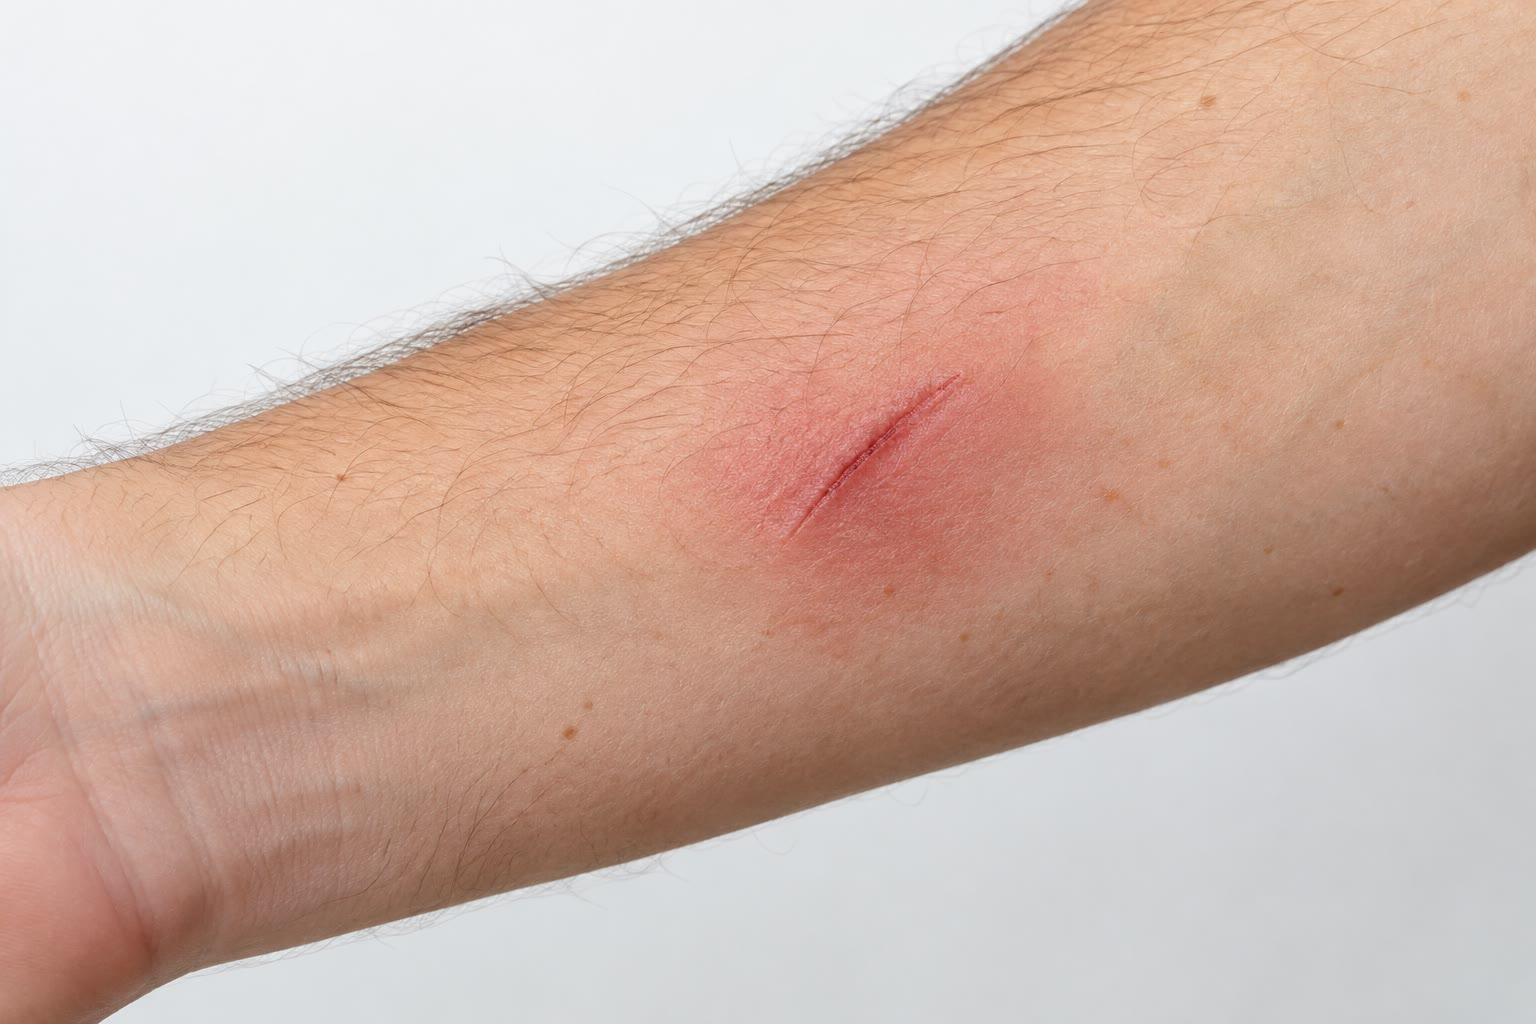
\includegraphics[width=0.52\linewidth]{images/book5/ai/b5-15-inflamed-skin.jpg}

{\small \omterm{def:b3:innate-immunity:inflammation}{Inflamação} aguda em volta de um arranhão de espinho: rubor e
calor dos vasos dilatados, inchaço do plasma vazado e a dor que mantém
o membro imóvel --- a resposta local que, generalizada ao corpo
inteiro, é o choque séptico.}
\end{omfigure}

\section{Matar}

\begin{definition}[Fagocitose e explosão respiratória]\label{def:b3:innate-immunity:killing}
\index{fagocitose}\index{explosão respiratória}\index{NADPH oxidase}\index{armadilha extracelular de neutrófilos}
Um fagócito prende sua presa por receptores de opsoninas --- a C3b e as
regiões constantes dos anticorpos --- ou diretamente por receptores de
padrões, envolve-a em membrana e fecha o \emph{fagossomo}, que se funde
com grânulos e \omterm{def:b3:membrane-traffic:endocytosis}{lisossomos}. A morte vem por vários meios ao mesmo tempo.
A \emph{explosão respiratória}: a enzima \emph{NADPH oxidase}, montada
na membrana do fagossomo, bombeia elétrons para o oxigênio e faz
superóxido, que vira peróxido de hidrogênio, que a mieloperoxidase
converte, com cloreto, em hipoclorito --- água sanitária, em
concentração milimolar, dentro de um compartimento de um micrômetro. O
óxido nítrico da NO sintase induzível, que com o superóxido dá
peroxinitrito. Ácido, até pH~5. Lisozima, proteases, lactoferrina que
priva a presa de ferro e defensinas que a perfuram. Um \omterm{def:b3:innate-immunity:innate}{neutrófilo} que
não consegue comer o que encontra --- uma hifa fúngica, um aglomerado
--- pode expelir sua própria \omterm{def:b3:chromatin-epigenetics:nucleosome}{cromatina} como uma rede pegajosa de DNA e
proteínas de grânulo, uma \emph{armadilha extracelular de \omterm{def:b3:innate-immunity:innate}{neutrófilos}},
e morrer ao fazê-lo. As crianças que herdam uma NADPH oxidase
defeituosa (doença granulomatosa crônica) sofrem abscessos e granulomas
de repetição por bactérias e fungos que fagócitos comuns matam sem
dificuldade: a explosão não é opcional.
\end{definition}

\begin{definition}[Células natural killer e interferon]\label{def:b3:innate-immunity:nk-ifn}
\index{célula natural killer!ausência do próprio}\index{interferon!tipo I}\index{estado antiviral}
Os \omterm{def:b3:virology:virus}{vírus} se escondem dentro das células, onde o \omterm{def:b3:innate-immunity:complement}{complemento} e os
fagócitos não os alcançam. As \emph{\omterm{def:b3:innate-immunity:innate}{células natural killer}} patrulham
em busca de células que pararam de exibir o MHC de classe~I --- a
``ausência do próprio'' de uma célula cujo ocupante viral ou tumoral
desligou a apresentação de antígeno para escapar das células T
(\cref{ch:b3:adaptive-immunity}) --- e de proteínas de estresse que
células infectadas e transformadas põem em sua superfície; receptores
inibitórios do MHC~I e receptores ativadores dos ligantes de estresse
são somados, e a célula que desequilibra a balança é morta em minutos
pela perforina e pelas granzimas injetadas nela, que disparam sua
\omterm{def:b3:cell-cycle-apoptosis:apoptosis}{apoptose}. Os \emph{interferons do tipo~I} ($\alpha$ e $\beta$) são
feitos por qualquer célula cuja RIG-I ou cGAS tenha detectado ácido
nucleico viral; secretados, ligam-se a receptores das células vizinhas
e, pela via JAK--STAT, induzem centenas de genes que põem essas células
num \emph{estado \omterm{def:b3:virology:drugs}{antiviral}}: uma quinase que desliga a tradução quando
encontra RNA de fita dupla, uma nuclease que degrada RNA, proteínas que
bloqueiam a entrada e a montagem virais, e mais MHC~I para mostrar às
células T o que há dentro. A célula que fez o interferon pode morrer;
suas vizinhas ficam avisadas. O interferon foi descoberto por Isaacs e
Lindenmann (1957) como o fator, presente no meio de células infectadas
por \omterm{def:b3:virology:virus}{vírus}, que tornava resistentes células novas, e é a razão pela qual
uma célula infectada por um \omterm{def:b3:virology:virus}{vírus} resiste a um segundo.
\end{definition}

\begin{method}[Medir a inflamação e a função dos fagócitos]\label{met:b3:innate-immunity:tests}
\index{proteína C reativa!dosagem}\index{teste do nitroazul de tetrazólio}
À beira do leito: (1) a \emph{\omterm{prop:b3:innate-immunity:systemic}{proteína C reativa}} no soro, por
imunoensaio --- abaixo de \qty{5}{mg/L} em repouso, dezenas numa
infecção viral, centenas numa sepse bacteriana, caindo em poucos dias
com tratamento eficaz; (2) a contagem de \omterm{def:b3:innate-immunity:innate}{neutrófilos}, elevada na
infecção bacteriana, com formas imaturas liberadas cedo pela medula;
(3) a velocidade de hemossedimentação, um substituto lento do
fibrinogênio. Para os fagócitos: (4) o teste do \emph{nitroazul de
tetrazólio} ou da di-hidrorrodamina, em que \omterm{def:b3:innate-immunity:innate}{neutrófilos} estimulados in
vitro reduzem um corante se sua \omterm{def:b3:innate-immunity:killing}{NADPH oxidase} funciona --- o
diagnóstico da doença granulomatosa crônica numa manhã; (5) um ensaio
de quimiotaxia, contando as células que migram através de um filtro em
direção a uma \omterm{def:b3:innate-immunity:inflammation}{quimiocina}.
\end{method}

\section{Da inata à adaptativa, e por toda a vida}

\begin{proposition}[A decisão da célula dendrítica]\label{prop:b3:innate-immunity:bridge}
\index{célula dendrítica!maturação}\index{coestimulação}\index{adjuvante}
A imunidade adaptativa não começa sozinha. Uma \emph{\omterm{def:b3:innate-immunity:innate}{célula dendrítica}}
num tecido come o que encontra; se seus receptores de padrões são
disparados --- por micróbio ou por dano ---, ela amadurece: para de
comer, migra pelos linfáticos até o linfonodo de drenagem, exibe em
moléculas de MHC os peptídeos daquilo que comeu e expõe moléculas
\emph{coestimuladoras} (B7) e \omterm{def:b3:innate-immunity:inflammation}{citocinas} que dizem a uma célula T que
reconheça o peptídeo para responder, e como
(\cref{ch:b3:adaptive-immunity}). Uma célula T que vê seu peptídeo numa
\omterm{def:b3:innate-immunity:innate}{célula dendrítica} sem coestimulação é desligada. O reconhecimento inato
decide, assim, se um antígeno merece uma resposta, e as \omterm{def:b3:innate-immunity:inflammation}{citocinas} que a
\omterm{def:b3:innate-immunity:innate}{célula dendrítica} faz --- decididas por quais receptores de padrões
dispararam --- decidem se a resposta é dirigida a \omterm{def:b3:virology:virus}{vírus}, bactérias ou
vermes. Um \emph{adjuvante} é um ligante de receptor de padrões
acrescentado a uma vacina para fornecer esse sinal; o alume e as
nanopartículas lipídicas das vacinas modernas funcionam por disparar
isso.
\end{proposition}

\begin{remark}[A imunidade inata em toda parte, e sua memória]\label{rem:b3:innate-immunity:everywhere}
Todo organismo multicelular tem \omterm{def:b3:innate-immunity:innate}{imunidade inata}, e as plantas, os
fungos e os invertebrados não têm outra coisa. As plantas reconhecem
flagelina e quitina com quinases receptoras e montam uma resposta em
dois níveis (\cref{ch:b3:plant-molecular-physiology}); os insetos têm
Toll e peptídeos antimicrobianos; até as bactérias têm \omterm{def:b3:genetic-engineering:tools}{enzimas de
restrição} e \omterm{def:b3:genetic-engineering:crispr}{CRISPR} (\cref{ch:b3:genetic-engineering}). O dogma de que a
\omterm{def:b3:innate-immunity:innate}{imunidade inata} não tem memória se abrandou: um monócito que encontrou
$\beta$-glicano ou a vacina BCG é epigeneticamente reprogramado
(\cref{ch:b3:chromatin-epigenetics}) para responder mais fortemente a
micróbios sem relação alguma durante meses --- a \emph{imunidade
treinada}, que explica por que o BCG reduz a mortalidade infantil por
infecções que não a tuberculose. E o excesso do sistema é uma doença do
nosso tempo: a \omterm{def:b3:innate-immunity:inflammation}{inflamação} estéril movida por cristais de ácido úrico
(gota), cristais de colesterol na parede arterial (aterosclerose),
\omterm{def:b3:structural-biology:amyloid}{amiloide} no cérebro, e a \omterm{def:b3:innate-immunity:inflammation}{inflamação} de baixo grau da obesidade e da
velhice.
\end{remark}

\section{Exercícios}

\begin{exercise}[$\star$]\label{exo:b3:innate-immunity:1}
Liste quatro \omterm{def:b3:innate-immunity:innate}{barreiras} e cinco tipos celulares da \omterm{def:b3:innate-immunity:innate}{imunidade inata}, com
uma função de cada.
\end{exercise}

\begin{exercise}[$\star$]\label{exo:b3:innate-immunity:2}
O que faz de uma molécula um bom \omterm{def:b3:innate-immunity:prr}{padrão molecular associado a
patógenos}? Dê três exemplos e o receptor de cada um.
\end{exercise}

\begin{exercise}[$\star$]\label{exo:b3:innate-immunity:3}
Explique cada um dos quatro sinais de Celso por um mediador e uma
alteração vascular ou neural.
\end{exercise}

\begin{exercise}[$\star$]\label{exo:b3:innate-immunity:4}
Nomeie as três vias do \omterm{def:b3:innate-immunity:complement}{complemento}, o que dispara cada uma e os três
desfechos da clivagem da C3.
\end{exercise}

\begin{exercise}[$\star\star$]\label{exo:b3:innate-immunity:5}
No modelo do \omterm{def:b3:innate-immunity:complement}{complemento} com $k_{0} = 2$ por segundo, $a =
\qty{0.15}{s^{-1}}$ e $d = \qty{0.05}{s^{-1}}$ sobre um micróbio,
quantas C3b são depositadas depois de \qty{60}{s}? E depois de
\qty{90}{s}? Sobre uma célula do hospedeiro com $a = 0.05$ e $d = 0.15$,
qual é o estado estacionário?
\end{exercise}

\begin{exercise}[$\star\star$]\label{exo:b3:innate-immunity:6}
Ordene os eventos do \omterm{def:b3:innate-immunity:inflammation}{extravasamento}, nomeie a classe de moléculas de
cada etapa e preveja o fenótipo de uma criança cujos \omterm{def:b3:innate-immunity:innate}{neutrófilos} não
têm \omterm{def:b3:innate-immunity:inflammation}{integrinas} $\beta_{2}$ (deficiência de adesão leucocitária).
\end{exercise}

\begin{exercise}[$\star\star$]\label{exo:b3:innate-immunity:7}
Os \omterm{def:b3:innate-immunity:innate}{neutrófilos} de um paciente falham no teste da di-hidrorrodamina.
Qual é o diagnóstico, que reação está faltando e que infecções você
espera? Por que se formam granulomas?
\end{exercise}

\begin{exercise}[$\star\star$]\label{exo:b3:innate-immunity:8}
Explique o reconhecimento da ausência do próprio e preveja o que
acontece com uma célula tumoral que (a) perde o MHC~I para escapar das
células T, (b) mantém o MHC~I mas exibe ligantes de estresse.
\end{exercise}

\begin{exercise}[$\star\star$]\label{exo:b3:innate-immunity:9}
Por que uma vacina de proteína pura induz pouca imunidade, e o que
acrescenta um adjuvante? Relacione com o argumento de Janeway.
\end{exercise}

\begin{exercise}[$\star\star\star$]\label{exo:b3:innate-immunity:10}
A febre custa \qty{12}{\%} do metabolismo de repouso por grau e retarda
a duplicação de uma bactéria de \qty{30}{min} a \qty{37}{\celsius} para
\qty{45}{min} a \qty{40}{\celsius}. Ao longo de um dia de infecção,
calcule a população bacteriana a partir de $10^{4}$ com e sem febre
(ignorando a morte), e a energia extra para uma pessoa de
\qty{8}{MJ/d}. A febre vale a pena? De que depende a resposta?
\end{exercise}

\begin{exercise}[$\star\star\star$]\label{exo:b3:innate-immunity:11}
Algumas bactérias ligam o fator H à sua superfície; outras clivam a C3b
ou descartam sua cápsula. Usando o \cref{thm:b3:innate-immunity:complement},
explique cada uma como uma mudança de $a$ ou de $d$, e diga qual é a
defesa mais econômica para o micróbio.
\end{exercise}

\begin{exercise}[$\star\star\star$]\label{exo:b3:innate-immunity:12}
Argumente, com os mecanismos deste capítulo, por que a mesma resposta é
adaptativa numa farpa e letal na corrente sanguínea, e por que os
fármacos que bloqueiam o TNF ajudam na artrite reumatoide mas aumentam
o risco de tuberculose.
\end{exercise}

\section{Problema: Uma Farpa}

\begin{problem}[{Problema de fim de semana --- dez mil bactérias sob a
pele em corrida contra os neutrófilos enviados ao seu encontro,
revestidas de complemento pela aritmética da alça, combatidas com febre
ao seu preço metabólico e, na corrente sanguínea, transformadas na
fisiologia do choque, terminando nas bactérias restantes após seis
horas, na C3b sobre cada uma e no custo de um dia de febre}]
\label{pb:b3:innate-immunity:1}
Dados: $10^{4}$ bactérias inoculadas, dobrando a cada \qty{40}{min}; os
\omterm{def:b3:innate-immunity:innate}{neutrófilos} chegam a partir de \qty{1}{h} a $2\times 10^{4}$ por hora,
cada um matando $20$ bactérias e depois morrendo. \omterm{def:b3:innate-immunity:complement}{Complemento}: $k_{0} = 1$ por segundo por bactéria, $a - d = \qty{0.08}{s^{-1}}$ sobre as
bactérias, $d - a =
\qty{0.1}{s^{-1}}$ sobre as células do hospedeiro;
a superfície de uma bactéria comporta no máximo $2\times 10^{6}$ C3b.
Febre: $+\qty{2}{\celsius}$ custa \qty{24}{\%} de um metabolismo de
\qty{8}{MJ/d} e alonga o tempo de duplicação bacteriano para
\qty{60}{min}. Sepse: $10^{9}$ bactérias em \qty{5}{L} de sangue,
$3\times 10^{6}$ moléculas de \omterm{def:b3:bacteriology:envelope}{lipopolissacarídeo} por bactéria; a
sinalização do TLR4 satura em $10^{-9}$ mol/L de \omterm{def:b3:bacteriology:envelope}{lipopolissacarídeo}.

\medskip
\noindent\textbf{Parte I --- A corrida.}
\begin{enumerate}
  \item Quantas bactérias há a \qty{1}{h}, quando chegam os primeiros
        \omterm{def:b3:innate-immunity:innate}{neutrófilos}, se nenhuma foi morta?
  \item Entre \qty{1}{h} e \qty{2}{h}, quantos \omterm{def:b3:innate-immunity:innate}{neutrófilos} chegam e
        quantas bactérias eles conseguem matar? Compare com o
        crescimento bacteriano nessa hora a partir da contagem da
        questão 1.
  \item Continue hora a hora (crescimento e, em seguida, morte ao fim de
        cada hora) até \qty{6}{h}. Quando a população atinge o pico e
        quantas restam a \qty{6}{h}?
  \item Refaça com uma chegada de \omterm{def:b3:innate-immunity:innate}{neutrófilos} atrasada para \qty{3}{h}.
        O que acontece até \qty{6}{h}? Comente o valor da rapidez.
  \item Quantos \omterm{def:b3:innate-immunity:innate}{neutrófilos} mortos se acumulam até o momento em que as
        bactérias desaparecem na questão 3? O que é o pus e por que ele
        precisa ser removido?
  \item Uma pessoa com um décimo da contagem normal de \omterm{def:b3:innate-immunity:innate}{neutrófilos}
        (neutropenia após quimioterapia): refaça a questão 3 e explique
        por que tais pacientes recebem \omterm{def:b3:bacteriology:antibiotics}{antibióticos} à primeira febre.
\end{enumerate}

\medskip
\noindent\textbf{Parte II --- O revestimento.}
\begin{enumerate}[resume]
  \item Pelo teorema, quantas C3b são depositadas sobre uma bactéria
        depois de \qty{30}{s}, \qty{60}{s} e \qty{120}{s}?
  \item Quando a superfície satura?
  \item Numa célula do hospedeiro ao lado dela, qual é o número
        estacionário de C3b?
  \item A bactéria adquire uma cápsula que reduz $a$ à metade, de modo
        que $a -
        d = 0.03$. Recalcule a C3b a \qty{120}{s}. O que a
        cápsula lhe compra?
  \item Quantas C3b carrega, na saturação, todo o inóculo de $10^{4}$
        bactérias, e que fração isso representa das $2\times 10^{16}$
        moléculas de C3 de um litro de plasma?
  \item Um paciente não tem C3. Que vias são afetadas e que infecções
        se seguem? Um paciente não tem C9: por que o fenótipo é mais
        brando e restrito a um único gênero?
\end{enumerate}

\medskip
\noindent\textbf{Parte III --- A febre.}
\begin{enumerate}[resume]
  \item Quanta energia extra custam dois dias de febre a
        $+\qty{2}{\celsius}$, em megajoules e em gramas de gordura
        (\qty{38}{kJ/g})?
  \item Refaça a questão 1 na temperatura de febre: quantas bactérias
        há a \qty{1}{h}? Por qual fator a febre reduziu a população que
        os \omterm{def:b3:innate-immunity:innate}{neutrófilos} encontram?
  \item No modelo da questão 3, com o tempo de duplicação mais longo,
        quando as bactérias desaparecem?
  \item A \omterm{prop:b3:innate-immunity:systemic}{proteína C reativa} sobe de \qty{1}{mg/L} para \qty{200}{mg/L}
        em dois dias. Com um volume plasmático de \qty{3}{L} e uma massa
        molecular de \qty{115}{kDa}, quantas moléculas o fígado
        produziu, e quantas por segundo?
  \item Os antipiréticos bloqueiam a síntese de prostaglandinas. O que
        fazem com o ponto de ajuste, com o conforto do paciente e, pelos
        números acima, com a infecção?
  \item Por que uma febre de \qty{41}{\celsius} é perigosa quando
        \qty{39}{\celsius} não é, e o que impede o ponto de ajuste de
        subir indefinidamente?
\end{enumerate}

\medskip
\noindent\textbf{Parte IV --- O choque.}
\begin{enumerate}[resume]
  \item Moléculas de \omterm{def:b3:bacteriology:envelope}{lipopolissacarídeo} no sangue do paciente séptico e
        sua concentração em mol/L.
  \item Compare com a concentração saturante para o TLR4. Todos os
        \omterm{def:b3:innate-immunity:innate}{macrófagos} do corpo estão ativados?
  \item Cada um dos $10^{11}$ \omterm{def:b3:innate-immunity:innate}{macrófagos} do corpo libera \num{1000}
        moléculas de TNF por segundo durante uma hora. Quantos moles de
        TNF, e que concentração em \qty{15}{L} de líquido extracelular?
        (O TNF age a \qty{1e-11}{mol/L}.)
  \item Explique a queda da pressão arterial e a falência dos rins a
        partir dos mecanismos locais da \omterm{def:b3:innate-immunity:inflammation}{inflamação}.
  \item O \omterm{def:b3:bacteriology:antibiotics}{antibiótico} dado na admissão mata as bactérias em uma hora.
        Por que o paciente pode piorar antes de melhorar, e o que limita
        a utilidade dos anticorpos anti-TNF na sepse?
  \item Uma linhagem de camundongos não tem TLR4. Preveja sua resposta
        ao \omterm{def:b3:bacteriology:envelope}{lipopolissacarídeo} injetado e a uma infecção viva por
        \omterm{def:b3:bacteriology:envelope}{Gram-negativas}, e explique o paradoxo aparente.
  \item Resuma: as bactérias restantes a \qty{6}{h} (questão~3), a C3b
        sobre uma bactéria a \qty{120}{s} (questão~7) e o custo de dois
        dias de febre (questão~13).
\end{enumerate}
\end{problem}
